\section{Reparametrizační trik}
\label{sec:reparametrization_trick}
Reparametrizační trik spočívá v přesunutí procesu vzorkování do vstupní vrstvy. \cite{Doersch2021}

Reparametrizační trik \emph{funguje} pouze pakliže lze vzorkovat z $Q(z\mid X)$ vyhodnocením funkce $h(\eta, X)$, kde $\eta$ je šum (z distribuce jejíž parametry nejsou učeny z dat). $h$ také musí být spojitá na $X$, abychom skrze něj mohli provádět zpětnou propagaci.
To, mimo jiné, znamená, že $Q(z\mid X)$ a tím padem i $P(z)$ \textbf{nemohou být diskrétní rozdělení}. V opačném případě by došlo k nespojitosti prostoru vzorků $Q$ – a tedy neschopnosti generativního modelu generovat vzorky v celém rozsahu, včetně vzorků které nebyl součástí dat (běžný problém autoenkodérů, které uvedla \autoref{chap:autoencoder}.)

Mějme $\mu(X)$ a $\Sigma(X)$. Pak je možné vzorkovat z $\mathcal{N}(\mu(X), \Sigma(X))$ – nejprve provedeme vzorkování z $\epsilon \sim \mathcal{N}(0, I)$ a následně spočteme $z = \mu(X) + \Sigma^{\frac{1}{2}}(X) * \epsilon$. \cite{Doersch2021}
Interpretaci hodnot $\mu$ a $\sigma$ nabízí enkodér a dekodér moduly modulu variačního autoenkodéru dle \autoref{sec:vae_model_architecture}.

Finální rovnice, jejíž gradient chceme spočítat má následující tvar:

\begin{equation} \label{eq:vae_reparam_trick}
    \mathds{E}_{X \sim D} \left[ \mathds{E}_{\mathcal{N}(\epsilon; 0, 1)} \left[ \log P(X\mid z = \mu(X) + \Sigma^{\frac{1}{2}} (X) * \epsilon) \right] -  D_{KL}(q_\phi(\textbf{z}\mid\textbf{x})\parallel p_\theta(\textbf{z})) \right].
\end{equation}

\begin{figure}[H]
    \centering
    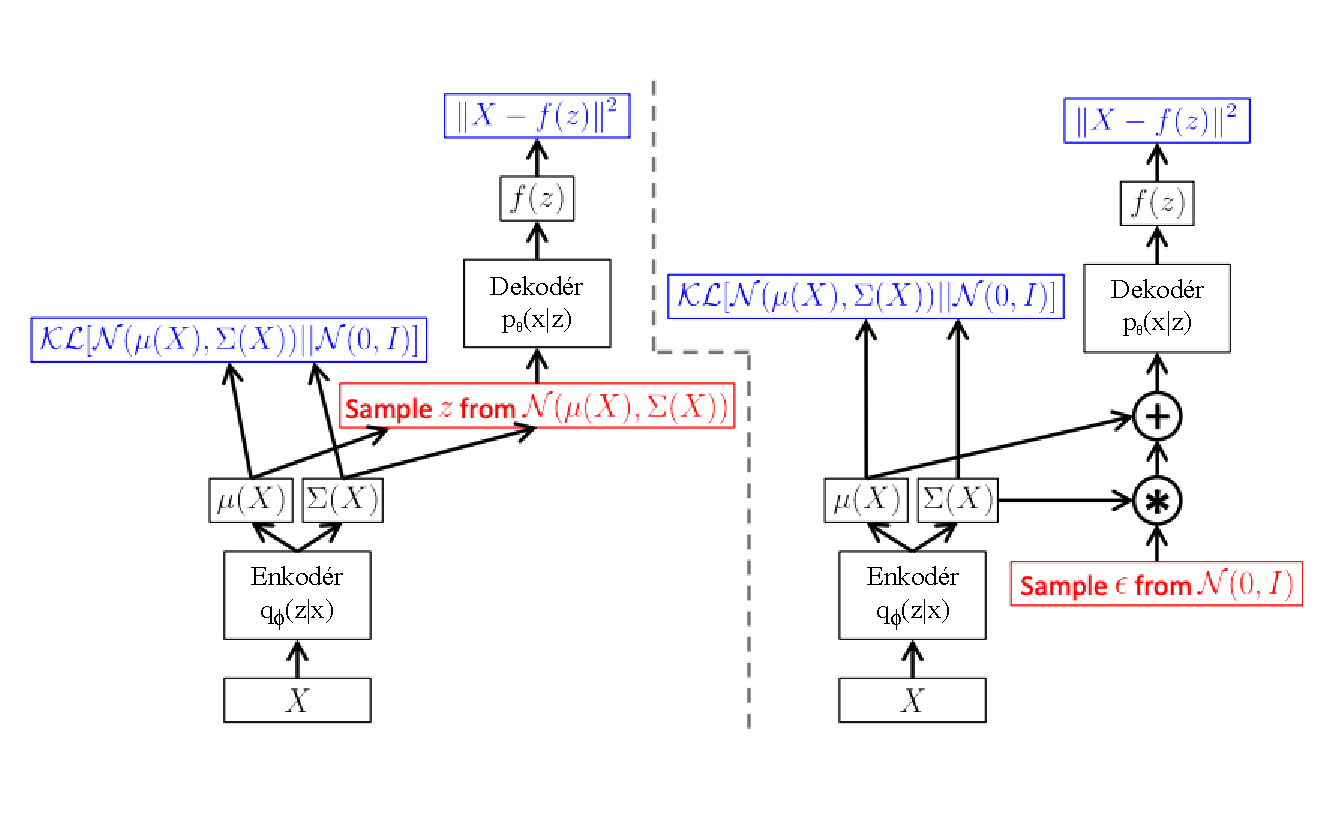
\includegraphics[width=0.8\textwidth]{figures/vae_backpropagation.pdf}
    \caption{Trénovací fáze dopředné umělé neuronové sítě VAE. Levý obrázek je znázorněn bez reparametrizačního triku. Pravý obrázek zahrnuje reparametrizační trik. Červené bloky zobrazují vzorkovací operace, které jsou nediferenciovatelné. Modré bloky zobrazují ztrátové vrstvy neuronové sítě. Dopředné chování obou sítí je \textbf{identické}, ale pouze v síti na pravém obrázku lze provést zpětná propagace. Obrázek včetně interpretace převzat z \cite{Doersch2021}.}
    \label{fig:vae_backpropagation}
\end{figure}

Kýžená vlastnost \autoref{eq:vae_reparam_trick} je, že v modelu její \textbf{umělé neuronové sítě lze provést zpětnou propagaci}
\footnote{Žádné střední hodnoty ($\mathds{E}$) \autoref{eq:vae_reparam_trick} \textbf{nezávisí} na parametrech modelu. Tedy do těchto středních hodnot můžeme bezpečně převést symbol gradientu a zároveň dodržet jejich rovnost. 
Tedy, mějme neměnné $X$ a $\epsilon$, pak je tato funkce \textbf{spojitá a deterministická} v parametrech $P$ a $Q$, což v důsledku znamená možnost zpětné propagace vypočíst gradient algoritmem stochastického gradientního sestupu.}. 
A díky tomu lze srkze model variačního autoenkodéru zpětně propagovat chyba ztrátové funkce a tím způsobem jej optimalizovat (viz \autoref{sec:multilayer_perceptron}). Toto znázorňuje \autoref{fig:vae_backpropagation}(b). \cite{Kingma2014}
